% Editable illustration of the two histories in supp:nonidentifiability.
% Shared-input description is in the manuscript caption.
% Build: make -C paper figure-nonidentifiability-v2
\documentclass[tikz,border=3pt]{standalone}
\usepackage[T1]{fontenc}
\usepackage{amsmath,amssymb}
\usetikzlibrary{arrows.meta,backgrounds}
\definecolor{CTBFnavy}{HTML}{27325E}
\definecolor{CTBFteal}{HTML}{2E7D78}
\definecolor{CTBForange}{HTML}{D8704A}
\begin{document}
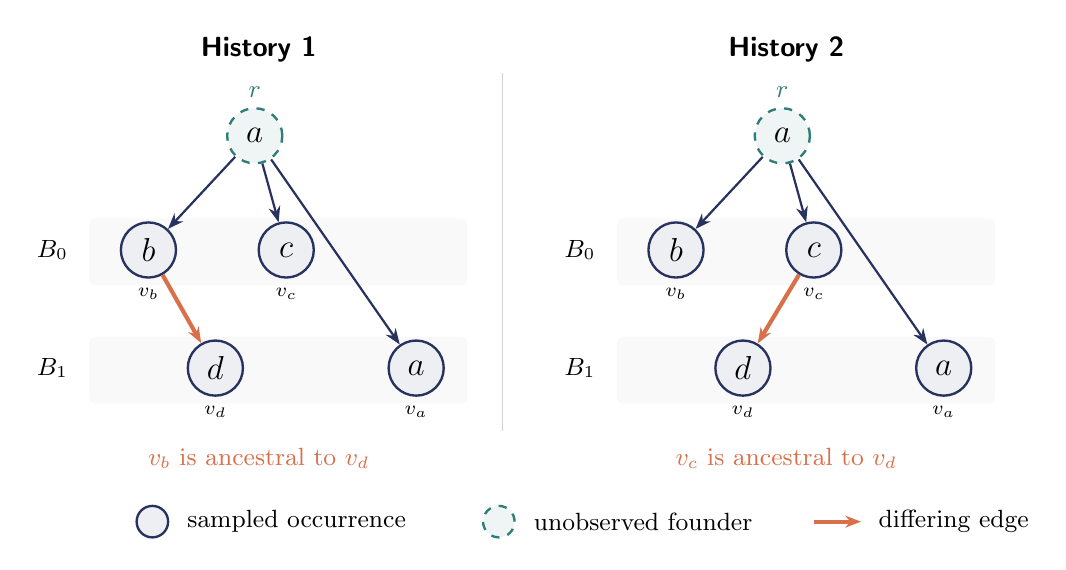
\begin{tikzpicture}[
  x=1cm,y=1cm,font=\sffamily,
  observed/.style={circle,draw=CTBFnavy,fill=CTBFnavy!8,
    line width=.85pt,minimum size=7mm,inner sep=0pt,font=\large},
  founder/.style={observed,draw=CTBFteal,fill=CTBFteal!8,dashed},
  ancestry/.style={-{Stealth[length=2mm]},draw=CTBFnavy,line width=.8pt},
  changed/.style={ancestry,draw=CTBForange,line width=1.5pt},
  smalltext/.style={font=\small,align=center},
  title/.style={font=\sffamily\bfseries\normalsize}
]
\foreach \offset/\which/\parent in {0/1/b,6.7/2/c}{
  \begin{scope}[xshift=\offset cm]
    \node[title] at (2.95,4.45) {History \which};
    \begin{scope}[on background layer]
      \fill[CTBFnavy!3,rounded corners=2pt] (.8,1.45) rectangle (5.6,2.3);
      \fill[CTBFnavy!3,rounded corners=2pt] (.8,-.05) rectangle (5.6,.8);
    \end{scope}
    \node[smalltext,anchor=east] at (.65,1.9) {$B_0$};
    \node[smalltext,anchor=east] at (.65,.4) {$B_1$};
    \node[founder,label={[font=\small,text=CTBFteal]above:$r$}]
      (r) at (2.9,3.35) {$a$};
    \node[observed,label={[font=\scriptsize]below:$v_b$}]
      (b) at (1.55,1.9) {$b$};
    \node[observed,label={[font=\scriptsize]below:$v_c$}]
      (c) at (3.3,1.9) {$c$};
    \node[observed,label={[font=\scriptsize]below:$v_d$}]
      (d) at (2.4,.4) {$d$};
    \node[observed,label={[font=\scriptsize]below:$v_a$}]
      (a) at (4.95,.4) {$a$};
    \draw[ancestry] (r) -- (a);
    \draw[ancestry] (r) -- (b);
    \draw[ancestry] (r) -- (c);
    \draw[changed] (\parent) -- (d);
    \node[smalltext,text=CTBForange] at (2.95,-.75)
      {$v_{\parent}$ is ancestral to $v_d$};
  \end{scope}
}
\draw[gray!35] (6.05,-.4) -- (6.05,4.15);
\node[observed,minimum size=4mm] (legendObs) at (1.6,-1.55) {};
\node[font=\small,anchor=west] at (1.92,-1.55) {sampled occurrence};
\node[founder,minimum size=4mm] (legendRoot) at (6,-1.55) {};
\node[font=\small,anchor=west] at (6.32,-1.55) {unobserved founder};
\draw[changed] (10,-1.55) -- (10.6,-1.55);
\node[font=\small,anchor=west] at (10.7,-1.55) {differing edge};
\end{tikzpicture}
\end{document}
